\begin{figure}[!htbp]
\centering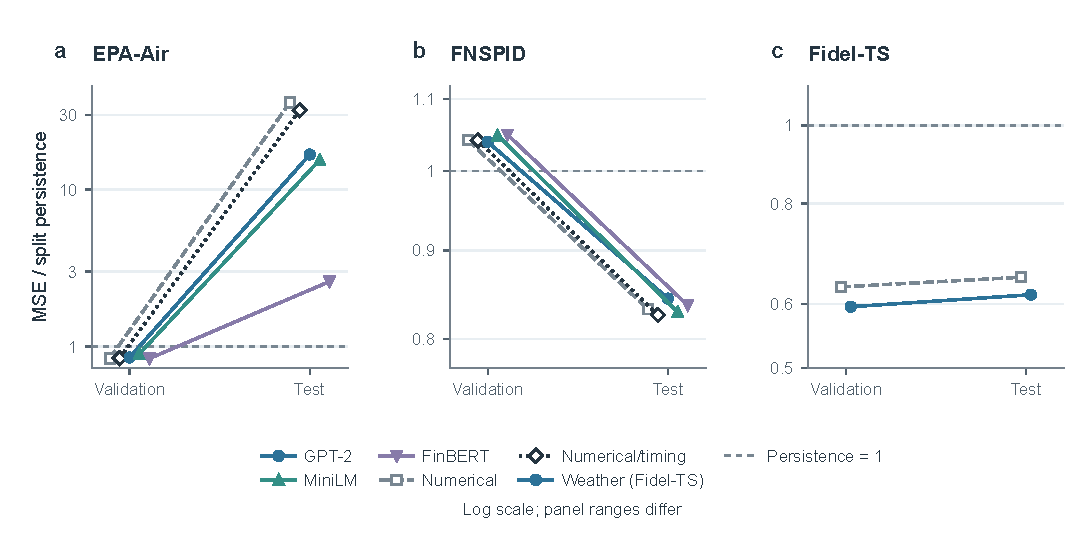
\includegraphics[width=\textwidth]{fig8_transfer}
\caption{Validation comparisons and later test transfer of independent ridge models. Pooled observed-scalar MSE is divided by persistence MSE from the same split; one is the baseline and lower is better. The vertical axis is logarithmic. EPA-Air and FNSPID include numerical, numerical/timing and three aligned text configurations; Fidel-TS includes numerical-only and aligned weather configurations relative to seasonal persistence. Each line connects one validation-selected state across splits. Ratios are descriptive transformations of saved means. Exact losses and penalties appear in Table~\ref{tab:ridge_capability_details}; perturbation contrasts appear in Table~\ref{tab:representations}.}
\label{fig:transfer}
\end{figure}

Validation comparisons and later test transfer are shown in Figure~\ref{fig:transfer}; fixed-model and retrained contrasts are reported in Table~\ref{tab:representations}.


A training-only probe on twelve financial direction sentences allowed MiniLM and FinBERT to classify all twelve differently phrased held-out sentences correctly. The probed direction is therefore recoverable within this vocabulary; forecasting performance requires separate evidence.

Replacement geometry also depends on a shared representation component. On FNSPID, GPT-2's median replacement cosine falls from 0.998964 to 0.188214 after subtracting the training centroid; MiniLM's falls from 0.454059 to 0.142177. On EPA-Air, FinBERT's median falls from 0.768842 to $-0.013962$. Raw cosine can thus be dominated by a shared direction and does not determine whether a task-relevant proposition changed.

On EPA-Air, all three content models improve the validation mean over persistence (1.075034). Only FinBERT improves over numerical/timing ridge (0.901160 versus 0.906853, a descriptive 0.63\% benefit). Every model loses to test persistence (0.751407), including numerical-only and numerical/timing ridge with MSEs of 27.056535 and 24.127104. Negative fixed-shuffle differences therefore accompany poor test-period transfer.

On FNSPID, persistence validation MSE is 0.648214, below numerical ridge (0.675381), numerical/timing ridge (0.675222) and all three content models (0.673852, 0.679578 and 0.680205). GPT-2's 0.20\% mean improvement over numerical/timing ridge thus provides no overall capability advantage. Later gains over test persistence (0.320936) cannot retrospectively qualify validation capability. No formal paired validation screen was applied to these representation comparisons.

Aggregation can reverse the effect's direction. For EPA-Air FinBERT, fixed shuffle reduces scalar-pooled MSE from 1.950746 to 1.945247 but increases entity-macro MSE from 2.388571 to 2.398929. Three of eight entities have a positive alignment point effect. FNSPID has 4/10 such entities for GPT-2, 2/10 for MiniLM and 4/10 for FinBERT. The pooled endpoint therefore need not represent a common entity-level direction.
